%\chapter{Procesos colisionales en átomos y moléculas simples}
\chapter{Ionización de átomos y moléculas simples}

%%%%%%%%%%%%%%%%%%%%%%%%%%%%%%%%%%%%%%%%%%%%%%%%%%%%%%%%%%%%%%%%%%%%%
\section{Introducción}
%%%%%%%%%%%%%%%%%%%%%%%%%%%%%%%%%%%%%%%%%%%%%%%%%%%%%%%%%%%%%%%%%%%%%

La exitosa idea de reemplazar la interacción no local de muchas 
partículas por una ecuación de un electrón abrió la posibilidad de 
estudiar sistemas extremadamente complejos con gran precisión.
En este contexto, el éxito de la teoría del funcional de la densidad
(\acs{dft}) \cite{HohenberKohn:64,KohnSham:65} despegó cuando avances 
cruciales en los términos de intercambio y correlación le dieron a la 
teoría poder predictivo para competir con métodos dependientes de 
funciones de onda hasta el momento bien estudiados~\cite{Becke:14}.
La importancia de los potenciales de intercambio y 
correlación en el mundo de la físico-química está particularmente
enfatizado en varios trabajos~\cite{Bartlett:10,Verma:12}.
En general, los potenciales de intercambio son construidos por 
aproximaciones locales al operador de intercambio de Hartree--Fock 
(\acs{hf}), i.e., el potencial de Slater~\cite{Slater:51}, el potencial 
efectivo optimizado (\acs{oep})~\cite{Sharp:53,Talman:76,Talman:89}, el 
potencial de Krieger--Li--Iafrate\cite{Krieger:92} y varios 
otros~\cite{Gorling:92,Yang:02,Staroverov:06,Ryabinkin:13}.

Por otro lado, el cálculo de procesos colisionales inelásticos requiere 
la correcta representación de los estados ligados y/o continuos 
involucrados en tales procesos. La existencia hipotética de un potencial 
efectivo local que permita la representación de dichos estados 
permitiría obtener las funciones de onda ortogonales de las partículas
intervinientes de manera más directa. Esta aproximación debería incluir
potenciales efectivos orbitales, una característica ausente en la 
mayoría de los métodos de funcional de la densidad existentes. 
Los métodos de pseudopotenciales tales como {\sc abinit}~\cite{abinit} 
o {\sc uspp}~\cite{Vanderbilt} no se pueden usar ya que éstos ignoran 
gran parte de la región interna de las funciones de onda. Estas regiones
contienen características del sistema que tienen un rol importante en
ciertos procesos colisonales, tales como la condición de cúspide en los 
procesos de captura electrónica e ionización. 

El problema inverso que supone la determinación de potenciales centrales 
a partir de funciones de onda y/o densidades electrónicas conocidas es 
una técnica bien estudiada en la comunidad de 
DFT~\cite{Wu:03,Gaiduk:13,Ryabinkin:15}. La extracción de los verdaderos
potenciales de intercambio--correlación de Kohn--Sham (\acs{ks}) a partir de 
densidades electrónicas casi exactas ha sido estudiada en sistemas de 
dos electrones tales como He~\cite{Mura:97}, iones de la secuencia 
electrónica de He~\cite{Umrigar:94}, y H$_2$\cite{Gritsenko:97,Mura:97},
así como también problemas con solución exacta (por ejemplo, el caso de
un potencial armónico externo~\cite{Filippi:94}).

Algunos trabajos, en donde se resuelve el problema inverso, los autores 
proponen un potencial de Kohn--Sham particular y resuelven el sistema
de ecuaciones correspondiente, obteniendo orbitales de 
KS~\cite{Schipper:97,deSilva:12,Kananenka:13}. A través de la inversión,
obtienen un potencial de KS reconstruido, que coincide con el original
en casi en toda su extensión excepto en algunas regiones cerca del 
origen, donde aparecen grandes oscilaciones. En algunos casos el 
potencial reconstruido está tan distorcionado que es imposible de 
reconocerlo~\cite{Mura:97,Jacob:11}. El mismo procedimiento fue 
sugerido hace varios años por Hilton \textit{et al.}, en aplicaciones
circunscriptas al cálculo de procesos de fotoionización en 
átomos~\cite{Hilton:77,Suzer:77}, agua~\cite{Hilton:79} y otras 
moléculas~\cite{Hilton:80,Crljen:87}. A su vez, estos trabajos se 
refieren a un trabajo previo en polarizabilidad atómica llevada a cabo 
por Sternheimer\cite{Sternheimer:54} y Dalgarno y 
Parkinson~\cite{Dalgarno:59}. Sin embargo, los autores se enfocaron en 
los resultados de secciones eficaces de fotoionización y no proveyeron 
detalles acerca de la calidad de los potenciales y las funciones de 
onda implementados.

En este contexto, emerge la idea del método de Inversión Depurada 
(\acs{dim})~\cite{Mendez:16,Mendez:18}, que permite la obtención de 
otenciales efectivos mediante la sustitución de las ecuaciones acopladas 
de muchos electrones por una ecuación de tipo Kohn--Sham. En primer 
lugar, los potenciales son obtenidos mediante la inversión directa de 
la ecuación de un electrón. Luego, se realiza una optimización, 
imponiéndo las condiciones de borde apropiadas de forma analítica. De 
esta manera, los potenciales DIM se parametrizan mediante simple 
expresiones.

En este capítulo, exploramos la posibilidad de implementar la 
aproximación del potencial efectivo en la teoría de colisiones atómicas 
para describir procesos inelásticos. En particular, examinaremos la 
ionización de atómos multielectrónicos y moleculas con pocos átomos por 
el impacto de protones y fotones. 
%diversos procesos colisionales que involucran transiciones de un electrón: fotoionización,excitación, ionización y captura. 
Una amplia variedad de métodos de primeros principios han sido 
implementados para el cálculo de secciones eficaces de ionización, 
desde las primeras implementaciones de la primera aproximación de Born (\acs{fba})~\cite{Bates:62,McDowell:61}, hasta los métodos más 
sofisticados de tratamiento totalmente mecanicocuántico 
\cite{Pindzola:07,Burke:11,Bray:17,Pindzola:16}. En el caso de 
blancos atómicos o moleculares, presentaremos resultados de secciones 
eficaces teóricas que serán comparadas con datos experimentales. No es 
nuestra intención hacer un repaso detallado de los métodos teóricos 
existentes, y ampliamente detallados en la bibliografía. El objetivo 
principal de este capítulo es ilustrar el uso efectivo de los 
potenciales DIM en aplicaciones colisionales. Para este fin realizaremos 
ciertas simplificaciones: 
\begin{enumerate}
\item Los cálculos están restringidos a los hamiltonianos que describen
sólo el proyectil, el blanco y el electrón activo;
\item Los elementos de matriz de transición se consideran en primer 
orden perturbativo. Si el primer orden fallase, no tendría sentido 
extender el cálculo a términos mayores de la serie. 
\end{enumerate}
Por simplicidad, restringiremos nuestros cálculos sólo se enmarca en
la FBA, que se conoce reproduce razonablemente las secciones eficaces
experimentales de diversos procesos en el rango de energía 
intermedio-alto del proyectil. Más aún, dentro de este rango de energía 
y orden de aproximación, se sabe que los orbitales de Hartree--Fock 
proporcionan el límite correcto a altas energías.

Examinaremos los procesos inelásticos mencionados anteriormente en 
el caso de tres átomos: litio, nitrógeno y neón. En este contexto,
inspeccionaremos la influencia de la descripción del blanco mediante
el potencial DIM en las secciones eficaces cuando la complejidad del 
blanco incrementa según el número de electrones.

Por otro lado, la descripción de sistemas moleculares constituye un 
verdadero desafío debido a su simetría no esférica y multicéntrica. 
Se han desarrollado un gran número de aproximaciones teóricas de 
primeros principios y semi-empríricas~\cite{Szabo:96,Helgaker:00,Schaefer:04} 
con este fin a lo largo de los años. Hacia el final de este capítulo, 
presentamos una extensión del método DIM para sistemas moleculares 
simples, proveyendo una nueva expresión paramétrica para potenciales 
moleculares. La descripción del blanco es examinada en procesos 
colisionales de primer orden, usando como ejemplo la molécula de metano 
a lo largo de dicho estudio.

\begin{comment}
Assuming the validity of the separation between exchange 
and correlation functionals, we will focus here only on the 
calculation of the exchange contribution to the potential.
Since Hartree--Fock does not include the correlations, 
our approach allows to obtain the ``exact''
one--electron local potential representing the exchange interactions. 
Strictly speaking, the method does not rely on the KS inversion formula 
since the Hartree--Fock solutions were the ones used for the inversion.
That is, we solved a KS--type equation, but rather than having 
KS--orbitals, we operated directly with the Hartree--Fock 
wavefunctions.
For open--shell atoms, we were able to find orbital 
spin--polarized exchange potentials, this being crucial, for 
instance, to find the hyperfine coupling 
constants\cite{Barone:94,Kaupp:10}.

However, this is not a simple task, and probably that is
why the method presented here has not been widely applied in the past. 
If the wavefunction has nodes, it will produce huge poles in the 
potential. 
Moreover, even for nodeless states, the asymptotic decaying behavior 
of the bound wavefunctions produces severe numerical difficulties, 
making the inversion operation intractable sometimes.
In our method, a depuration procedure follows the inversion. 
This depuration implies, first, the annihilation of the poles.
Then, a careful optimization of the potential which 
ensures the fulfillment of the appropriate boundary conditions. 

The work is organized as follows. 
Section \ref{sec:theory} describes the method, which includes 
the inversion procedure (\ref{subsec:directinversion}), 
the potential depuration (\ref{subsec:depuration}) and its further 
optimization (\ref{subsec:optimization}).
Section \ref{sec:results} presents the resulting effective potentials 
for the orbitals corresponding to the ground states of different 
noble gases, including a thorough 
examination of the wavefunctions generated by these potentials 
(\ref{subsec:resultsDIM}).
The corresponding exchange potentials are discussed in 
(\ref{subsec:exchange}), comparing the potentials for 
specific--$nl$ orbitals with averaged potentials.
Results of the same calculations for the Nitrogen atom are provided in
(\ref{subsec:Nitrogen}).
Atomic units are used unless otherwise specified.

\end{comment}

%%%%%%%%%%%%%%%%%%%%%%%%%%%%%%%%%%%%%%%%%%%%%%%%%%%%%%%%%%%%%%%%%%%%%
\section{El método de la inversión depurada}
%%%%%%%%%%%%%%%%%%%%%%%%%%%%%%%%%%%%%%%%%%%%%%%%%%%%%%%%%%%%%%%%%%%%%
\label{sec:dimatomos}

El método de inversión depurada consiste en suponer que los orbitales
de átomos multielectrónicos pueden ser representados por las soluciones
de un sistema de ecuaciones de un electrón activo para el cual existe 
un potencial efectivo que gobierna la dinámica del átomo.
Suponiendo que las funciones de onda $u_{nl}$, que representan las 
soluciones de la ecuación (\ref{eq:Schrodinger}), pueden ser aproximadas 
por funciones de onda de Hartree--Fock (HF) $u_{nl}^{\mathrm{HF}}$;
entonces, existe un potencial efectivo local correspodiente 
$V_{nl}^{\mathrm{HF}}$ que genera tales funciones de onda. Así, 
mediante esta suposición, convertimos el método de HF en un conjunto 
de ecuaciones de Kohn--Sham cuyas soluciones son las funciones de 
onda de Hartree--Fock,
\begin{equation}
\left[ 
-\frac{1}{2}\frac{d^{2}}{dr^{2}} + \frac{l(l+1)}{2r^{2}} + 
V_{nl}^{\mathrm{HF}}(r) 
\right] u_{nl}^{\mathrm{HF}}(r)
   = \varepsilon_{nl}^{\mathrm{HF}}\, u_{nl}^{\mathrm{HF}}(r) \, .
\label{eq:KS}
\end{equation}
A su vez, y debido a la naturaleza de las soluciones, el potencial 
efectivo generador
\begin{equation}
V_{nl}^{\mathrm{HF}}(r) = V^{\mathrm{ext}}(r) + 
V^{\mathrm{dir}}(r) + V_{nl}^{\mathrm{int}}(r) \, ,  
\label{eq:veff}
\end{equation}
está compuesto por un potencial externo $V^{\mathrm{ext}}$, 
el potencial directo o de Hartree $V^{\mathrm{dir}}$, y el potencial
de intercambio orbital $V_{nl}^{\mathrm{int}}$. A diferencia de los
potenciales más generales, este potencial no tiene el término de 
correlación electrónica ya que las soluciones de Hartree--Fock no lo 
incluyen. En el caso de un átomo en fase gaseosa, el potencial externo 
está queda determinado por el campo coulombiano del núcleo, mientras 
que el potencial de Hartree constituye la repulsión electrostática 
electrónica. 


%%%%%%%%%%%%%%%%%%%%%%%%%%%%%%%%%%%%%%%%%%%%%%%%%%%%%%%%%%%%%%%%%%%%%
\subsection{La inversión directa}
%%%%%%%%%%%%%%%%%%%%%%%%%%%%%%%%%%%%%%%%%%%%%%%%%%%%%%%%%%%%%%%%%%%%%
\label{subsec:inversion}

Dado que las funciones de onda $u_{nl}^{\mathrm{HF}}$ y energía orbitales 
$\varepsilon^{\mathrm{HF}}$ de Hartree--Fock son conocidas (calculadas 
numéricamente con los códigos {\sc hf} de C. F. Fischer~\cite{FroeseFischer:97}, 
y {\sc nrhf} de W. Johnson~\cite{Johnson:07}), es posible implementar 
la inversión directa de la ecuación (\ref{eq:KS}). Así, obtenemos el 
\textit{potencial invertido HF} 
\begin{equation}
V_{nl}^{\mathrm{HF}}(r) = 
\frac{1}{2}\frac{1}{u_{nl}^{\mathrm{HF}}(r)}
\frac{d^2}{dr^{2}}u_{nl}^{\mathrm{HF}}(r) - 
\frac{l(l+1)}{2r^{2}}+\varepsilon _{nl}^{\mathrm{HF}} \,,
\label{eq:VHF}
\end{equation}
el cual queda totalmente determinado por las soluciones 
$u_{nl}^{\mathrm{HF}}$ y $\varepsilon_{nl}^{\mathrm{HF}}$.

Inspeccionando el comportamiento de los potenciales invertidos, notamos 
que éstos tienen una forma coulombiana. Suponiendo que todos los 
potenciales invertidos siguen este comportamiento, ilustrado a la 
izquierda de la figura~\ref{fig:potycharge}, es conveniente definir una 
\textit{carga invertida HF} 
\begin{equation}
Z_{nl}^{\mathrm{HF}}(r) \equiv -r \, V_{nl}^{\mathrm{HF}}(r) \,.
\label{eq:Zeff}
\end{equation}
Esta carga efectiva, esquematizada del lado derecho de la 
figura~\ref{fig:potycharge}, deberá cumplir con condiciones de borde 
definidos por la naturaleza del blanco a describir. Esto es, en el 
origen la carga deberá ser igual a la carga nuclear del átomo, mientras 
que asintóticamente la carga debe ser igual a uno, debido al 
apantallamiento electrónico.

\begin{figure}[t!]
\centering
\includegraphics[width=0.9\textwidth]{dim/pot-charge.eps}
\caption[Características físicas del potencial y carga efectiva.]
{Ilustración de las características físicas esperadas del (a) potencial 
y (b) carga efectiva del blanco.}
\label{fig:potycharge}
\end{figure}

%%%%%%%%%%%%%%%%%%%%%%%%%%%%%%%%%%%%%%%%%%%%%%%%%%%%%%%%%%%%%%%%%%%%%
\subsection{Dificultades de la inversión directa}
%%%%%%%%%%%%%%%%%%%%%%%%%%%%%%%%%%%%%%%%%%%%%%%%%%%%%%%%%%%%%%%%%%%%%
\label{subsec:difnumericasDIM}

A pesar que el procedimiento de inversión de la ecuación~(\ref{eq:VHF}) 
es directo, éste no está libre de serias dificultades numéricas. 
La inversión de funciones de onda de Hartree--Fock tiene asociada tres
defectos que surgen de las características propias del método; los nodos 
genuinos no son estrictamente puntos de inflexión, el decaimiento 
exponencial de los orbitales sigue el comportamiento orbitales tipo 
Hartree, mientras que el método autoconsistente conduce a la aparición 
de nodos espúreos. 

\begin{figure}[t]
\centering
\includegraphics[width=0.9\textwidth]{dim/dim_2sK.eps} 
\caption[Función de onda radial y carga efectiva correspondiente.]
{(a) Función de onda radial $u_{2s}^{\mathrm{HF}}$ 
correspondiente al estado fundamental del átomo de potasio.
La función presenta dos nodos; un nodo genuino en $r \approx 0.111$~a.u. 
y un nodo espurio en $r\approx 5.75$~a.u. (ver recuadro). 
(b) Línea discontinua: carga efectiva invertida $Z_{2s}^{\mathrm{HF}}$, 
estropeada por la presencia de polos y divergencias.
Línea sólida: carga efectiva invertida depurada $Z_{2s}^{\mathrm{DIM}}$.}
\label{fig:2sK}
\end{figure}

Examinaremos estas dificultades numéricas y su trasfondo teórico 
inspeccionando un ejemplo que cuenta con todos los defectos que hemos 
encontrado. En la figura~\ref{fig:2sK} se muestra (a) la función de 
onda $u_{2s}^{\mathrm{HF}}$ del orbital $2s$ del átomo de potasio en su 
estado fundamental y (b) su correspondiente carga invertida 
$Z_{2s}^{\mathrm{HF}}$ (linea discontinua). La función de onda tiene un 
nodo genuino en $r\approx 0.111$~a.u., el cual es traducido a la carga 
efectiva invertida como un polo. La aparición de este polo sugiere que 
la función de onda en el denominador de la ecuación~(\ref{eq:VHF}) y su 
derivada segunda no se anulan entre sí en el nodo de la función. En la 
figura~\ref{fig:wave2sK} se muestran el orbital de HF y su segunda 
derivada numérica escaleada por un factor. 


\begin{figure}
\centering
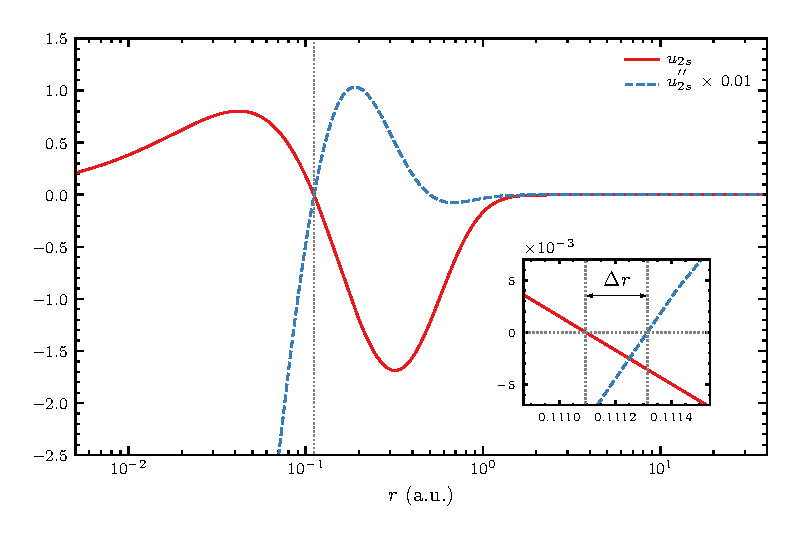
\includegraphics[width=0.9\textwidth]{dim/wave_2sK.eps} 
\caption[Función de onda radial y su derivada segunda de K.]
{Función de onda radial $u_{2s}^{\mathrm{HF}}$ y su derivada segunda 
del orbital $2s$ del átomo de potasio.}
\label{fig:wave2sK}
\end{figure}

\begin{figure}
\centering
\includegraphics[width=0.9\textwidth]{dim/dr_2sK.eps} 
\caption[Dependecia de $\Delta r$ del orden de aproximación numérica.]
{Dependecia de $\Delta r$ del orden de aproximación numérica en el 
orbital $2s$ del átomo de potasio.}
\label{fig:dr2sK}
\end{figure}

\begin{figure}
\centering
\includegraphics[width=0.9\textwidth]{dim/Lns_K.eps} 
\caption[$L_{nl}$.]
{$L_{nl}$ de los orbitales $s$ del átomo de K.}
\label{fig:dr2sK}
\end{figure}

\vspace{1cm}


\noindent
{\bf \color{red} Falta desarrollar.}

\begin{comment}
Por otro lado, todas las funciones de ondas 
de los electrones ligados decaen exponencialmente para distancias 
mayores al punto de retorno clásico. El punto de retorno clásico se 
define como la posición $r_{rc}$ en la cual la energía es igual al 
potencial efectivo. 

\begin{equation}
\lim_{r\rightarrow\infty} u_{nl}^{\mathrm{HF}}
= \exp\left(\sqrt{-2\varepsilon_{nl}^{\mathrm{HF}}} r\right)
\end{equation}

\begin{equation}
L_{nl}(r) \equiv r\frac{d\log u_{nl}}{dr}
\end{equation}

Este comportamiento ha llevado al consenso general de que el método 
de inversión sólo puede implementarse en orbitales sin 
nodos~\cite{Kananenka:13}. Por otro lado, una dificultad numérica menos 
obvia está dada por la razón entre la 
derivada de la función de onda y la función de onda en sí. 
{\color{red} Escribir sobre el primer paper de Adv. Quant. Chem y sobre 
la respuesta al comment de Cinal.}


At first glance, it seems that the turning point of $u_{2s}$ 
is located around $r_{tp} \approx 0.25$, and from that point on,  
the wavefunction should start to decay exponentially.
From the numerically point of view, say $r \approx 10 \, r_{tp}$ is 
a good point to stop the inversion, since beyond there, the effective 
charge could begin to diverge.


Thus, naively, one might infer that by erasing the points belonging 
to the neighborhood of the first node, and by stopping the inversion 
about $10 \, r_{tp}$, the inversion procedure 
will work well.
However, the dashed curve in Fig.~\ref{fig:2sKr}(b) shows a 
completely unphysical $Z^{\mathrm{HF}}_{2s}$ resulting from the 
inversion.
A very careful examination of the $u_{2s}^{\mathrm{HF}}$ orbital 
function evidences the presence of a spurious node at $r=1.51$ a.u., 
in a region where the amplitude of the wavefunction is 
less than $10^{-4}$ times the maximum value (see the 
inset of Fig. \ref{fig:2sKr}(a)).
Even though this node is completely innocuous for practical matters,  
it produces devastating effects in the inversion procedure, 
evidenced in the second huge peak in the 
$Z_{2s}^{\mathrm{HF}}$ curve (see Figure \ref{fig:2sKr}(b)). 
This pole is so big that affects a 
broad vicinity and causes the abrupt rising of the effective charge 
for $r>0.5$ a.u.. This is really a surprising result since 
{\it a priory} there is no reason to suspect that a negligible 
oscillation in the tail of the wavefunction would produce such a 
big drawback at such a small distance as 0.5 a.u.. 
Care must be taken then to discard such an undesired effect.

\textit{Second}, numerical rounding off of the exponential 
decay of the bound states hinders the corresponding inverted 
potential from having the physically desired asymptotic form. 
Moreover, there is a \textit{third} problem and this is at the heart 
of the Hartree Fock method: the exact solutions may have oscillations 
(and therefore, spurious nodes) in the large--r or ``tail'' region of 
the functions. 
The existence of these spurious nodes in Hartree Fock was already 
suggested by Fischer \cite{FroeseFischer:97}. 
This failure is not rooted in the numerical scheme but it is 
inherent to the method. Probably, these nodes are surviving 
long--range exchange effects due to the non--local character of the 
Hartree--Fock wavefunctions: the behavior of a particular orbital 
depends on all others. 
We have found the same spurious nodes at the same places even by 
using the different numerical codes.
As a general rule, the spurious nodes appear at very long distances, 
a region in which the amplitude of the wavefunction is very small. 
Therefore, their existence has no practical consequences, and they 
can be neglected in any general Hartree--Fock calculation.  
However, this is not true as far as the inversion procedure is 
concerned, as we will discuss in the next section.
\end{comment}

\newpage
%%%%%%%%%%%%%%%%%%%%%%%%%%%%%%%%%%%%%%%%%%%%%%%%%%%%%%%%%%%%%%%%%%%%%
\subsection{Método de depuración}
%%%%%%%%%%%%%%%%%%%%%%%%%%%%%%%%%%%%%%%%%%%%%%%%%%%%%%%%%%%%%%%%%%%%%
\label{subsec:depuracion}

Las dificultades numéricas mencionadas anteriormente convierten la 
obtención de potenciales $V_{nl}^{\mathrm{HF}}$ mediante la ecuación 
(\ref{eq:VHF}) en una tarea muy difícil. Para poder superar estas 
dificultades, hemos desarrollado el método de depuración, el cual 
consiste en optimizar cargas efectivas en lugar de potenciales efectivos. 
Así, somos capaces de restringir los valores de cualquier potencial a 
tener las condiciones de borde correctas, forzando el comportamiento de 
la carga efectiva invertida según
\begin{equation}
Z_{nl}^{\mathrm{DIM}}(r) \, \rightarrow 
\bigg\{ 
\begin{array}{ll}
Z_{N}  \ \  & \ \ \text{as\ \ }r  \rightarrow 0\  \\ 
1           & \ \ \text{as\ \ }r  \rightarrow \infty \ 
\end{array}\,,
\label{eq:Zasympt}
\end{equation}
donde $Z_N$ es la carga nuclear del blanco atómico. Una vez que se 
define la carga en los bordes, podemos obtener una expresión analítica
suave para $Z_{nl}^{\mathrm{DIM}}$, ajustando $Z_{nl}^{\mathrm{HF}}$ en
el mayor rango posible, exceptuando las zonas de comportamiento errático.
Estas condiciones se pueden cumplir imponiendole a la carga efectiva 
DIM que siga la expresión analítica dada por
\begin{equation}
Z_{nl}^{\mathrm{DIM}}(r)= \sum_{j=1}^{n} z_j e^{-\alpha_j r}+1 \,,
\label{eq:atomzDIM}
\end{equation}
donde $\Sigma_j z_j=Z_N-1$. Luego, los parámetros $z_j$ y $\alpha_j$ 
son optimizados de manera tal que reproduzcan las soluciones de HF de 
manera precisa.

%%%%%%%%%%%%%%%%%%%%%%%%%%%%%%%%%%%%%%%%%%%%%%%%%%%%%%%%%%%%%%%%%%%%%%%%
\subsubsection{Optimización de la carga DIM}
%%%%%%%%%%%%%%%%%%%%%%%%%%%%%%%%%%%%%%%%%%%%%%%%%%%%%%%%%%%%%%%%%%%%%%%%
\label{subsec:optDIM}

\begin{figure}[t]
\centering
\begin{tikzpicture}[remember picture]
%  \tikzset{shift={(current page.center)}}
  \node[process] (inv) {Inversión directa};
  \node[process] (rem) at (inv) [xshift=0cm,yshift=-1.5cm] 
            {Remoción de divergencias};
  \node[process] (eqnorm) at (rem) [xshift=0cm,yshift=-1.5cm] 
            {Ecuación normal};
  \node[process] (var) at (eqnorm) [xshift=0cm,yshift=-1.5cm] 
            {Variación de parámetros};
  \node[process] (diag) at (var) [xshift=-2.5cm,yshift=-2.3cm] 
            {Diagonalización};
  \node[process] (costo) at (var) [xshift=2.5cm,yshift=-2.3cm] 
            {Cálculo de costo};
  \node[decision] (converge) at (costo) [xshift=4cm,yshift=0cm] 
            {¿Convergió?};
  \node[process, fill=blue!20] (dim) at (converge) [xshift=0cm,yshift=-3.2cm] 
            {Potencial DIM};
  \draw [arrow] (inv) -- (rem);
  \draw [arrow] (rem) -- (eqnorm);
  \draw [arrow] (eqnorm) -- (var);
  \draw [arrow, bend right=33] 
            (var.west) 
            to ([xshift=-0.5cm,yshift=0cm]{diag.north});
  \draw [arrow, bend right=53] 
            ([xshift=-0.25cm,yshift=0cm]{diag.south}) 
            to ([xshift=0.25cm,yshift=0cm]{costo.south});
  \draw [arrow, bend right=33] 
            ([xshift=0.5cm,yshift=0cm]{costo.north}) 
            to (var.east);
  \draw [arrow, dashed] (costo) -- (converge);
  \draw [arrow, dashed] (converge) |- (rem.east) node [near start,left] {No};
  \draw [arrow, dashed] (converge) -- (dim.north)  node [midway,right] {Sí};
\end{tikzpicture}
\caption{Procedimiento de optimización del potencial DIM.}
\label{fig:procedimientoDIM}
\end{figure}

Un asunto muy importante en la optimización del potencial está dado 
por la autoconsistencia dentro de los códigos numéricos implementados
para el cálculo de las soluciones, y en particular los códigos usados
para la generación de las funciones de onda a ser invertidas. Para 
tal fin, hemos estudiado los códigos de Hartree--Fock 
\cite{FroeseFischer:97,Johnson:07} y hemos implementado las grillas
numéricas específicas de cada código, incluyendo los mismos métodos 
para el cálculo de derivadas. 

El ajuste del conjunto de parámetros $\left\{z_j,\alpha_j\right\}$ 
requiere un gran nivel de experiencia y detalle. El procedimiento 
general de la obtención de los potenciales DIM se esquematiza en la 
figura~\ref{fig:procedimientoDIM}. La clave de una optimización exitosa 
está dada por la definición de la región de ajuste: tiene que ser lo más 
extensa posible pero descartando los puntos cercanos a los polos y 
divergencias. De esta manera, la carga DIM $Z_{nl}^{\mathrm{DIM}}$ se 
superpone con la carga invertida $Z_{nl}^{\mathrm{HF}}$ a lo largo de 
la región interna bien comportada, permitiendo un ajuste preciso. La 
segunda parte de la optimización consiste en la obtención de una semilla 
para los parámetros $\left\{z_j,\alpha_j\right\}$. Estos valores son 
obtenidos mediante la resolución de la ecuación normal definida por el 
problema (ver detalles en anexo~\ref{app:ecnormal}). Los valores de las 
semillas obtenidas definen un potencial efectivo. A partir de esta 
potencial de prueba, se resuelve la ecuación dada por 
(\ref{eq:Schrodinger}), obteniendo las soluciones correspondientes. Las 
soluciones obtenidas nos permiten definir una función de costo definida 
previamente, la cual es minimizada repitiendo el procedimiento de forma 
iterativa. 

Es importante remarcar que la mayoría de los métodos de funcional de 
la densidad están basados en un principio variacional que minimiza el
funcional de energía. Sin descartar su importancia, la energía es solo
uno de los observables que caracteriza un estado cuántico. Más aún, a 
partir de diferentes funciones de prueba (de formas variadas) e 
implementando un método variacional, es posible reproducir la misma 
energía final. Un simple ejemplo es dado por 
Bartschat~\cite{Albright:93,Bartschat:96}, en donde dos potenciales
diferentes (uno conteniendo intercambio electrónico y otro despreciándolo)
conducen a energías similares y precisas de la serie de Rydberg en 
varios sistemas de cuasi-un electrón. Sin embargo, examinando estos 
potenciales éstos muestran grandes discrepancias cuando son implementados
en cálculos de dispersión \cite{BartschatBray:96}. Por lo tanto, además
de los valores de energía, hemos incluido en nuestra optimización 
valores medios de $\langle r^{n} \rangle$, tal que $n=-1,1$. La inclusión
de estos observables nos permite caracterizar la precisión de la función
de onda DIM acerca ($n=-1$) y lejos ($n=1$) del origen. Así, la función 
de costo que define nuestra optimización está dada por los errores 
relativos de cada una de estas cantidades
\begin{equation}
J=\sum_X \frac{X^{\mathrm{HF}}-\widebar{X}}{X^{\mathrm{HF}}}\,,
\end{equation}
donde la suma se hace sobre $X=\left[E,\langle r \rangle,\langle 1/r \rangle\right]$,
siendo $X^{\mathrm{HF}}$ los valores de HF y $\widebar{X}$ los 
resultados obtenidos de la diagonización del potencial de prueba. 

A partir de este procedimiento se obtiene la carga invertida depurada 
$Z_{2s}^{\mathrm{DIM}}(r)$ correspondiente al orbital $2s$ del átomo 
de potasio que se muestra con línea sólida en la figura~\ref{fig:2sK}(b).
Como se ve en la figura, se satisfacen las condiciones de borde dadas por
la ecuación~\ref{eq:Zasympt}, donde en el origen $Z_{2s} = 19$, y 
asintóticamente $Z_{2s} \rightarrow 1$.

%%%%%%%%%%%%%%%%%%%%%%%%%%%%%%%%%%%%%%%%%%%%%%%%%%%%%%%%%%%%%%%%%%%%%%%%
\section{Potenciales moleculares}
%%%%%%%%%%%%%%%%%%%%%%%%%%%%%%%%%%%%%%%%%%%%%%%%%%%%%%%%%%%%%%%%%%%%%%%%
\label{sec:potmoleculares}

En esta sección, el método de la inversión depurada es extendido para 
la obtención de potenciales efectivo moleculares. A continuación, 
utilizaremos la molécula de metano como ejemplo para mostrar la 
implementación del método.

Sin pérdida de generalidad, presentamos las bases teóricas para la 
obtención de potenciales moleculares DIM de compuestos de hidruro.
El hamiltoniano de un sistema de $N$--electrones de una molécula de 
tipo $X\!H_n$ dentro de la aproximación de Born--Oppenheimer (\acs{boa})
está dado por
\begin{equation}
 \mathcal{H}=-\sum_{i=1}^N \frac{1}{2} \nabla^2_{\mathbf{r}_i} 
 - \sum_{i=1}^N \frac{Z_N}{r_i} 
 + \sum_{i=1}^N V_H(r_i)
 + \sum_{i<j}^N \frac{1}{r_{ij}}\,,
\end{equation}
\begin{equation}
 V_H(r_i)=-\sum_{j=1}^{n} \frac{1}{\left|\mathbf{r}_i-\mathbf{R}_{H_j}\right|}\,,
\end{equation}
donde $Z_N$ es la carga nuclear del átomo más pesado $X$, y 
$\mathbf{R}_{H_j}$ son las coordenadas de los hidrógenos respecto al 
átomo $X$. La ecuación de Schr\"odinger correspondiente 
$\mathcal{H}\Psi=E\Psi$ se resuelve y, considerando la expansión de un 
centro (\acs{sce}), los orbitales se expresan según la 
ecuación~(\ref{eq:centralfield-wave}). Los orbitales y energías se 
encuentran resolviendo las ecuaciones de Hartree--Fock. El cálculo de 
estas ecuaciones generalmente recaen en el uso de conjuntos de bases 
(\acs{bs}) finitas para la representación de los orbitales moleculares 
(\acsp{mo}). Usualmente, los MOs son expresados como una combinación 
lineal de orbitales atómicos (\acs{lcao}), 
\begin{equation}
 \Psi_i=\sum_j c_{ji} \phi_j\,.
\end{equation}
A su vez, los orbitales atómicos pueden ser construidos a partir de 
conjuntos de base de orbitales tipo Gaussianos (\acsp{gto}).

%%%%%%%%%%%%%%%%%%%%%%%%%%%%%%%%%%%%%%%%%%%%%%%%%%%%%%%%%%%%%%%%%%%%%%%%
\subsection{Inversión y depuración con bases gaussianas}
%%%%%%%%%%%%%%%%%%%%%%%%%%%%%%%%%%%%%%%%%%%%%%%%%%%%%%%%%%%%%%%%%%%%%%%%
\label{subsec:invdepGTO}

La expresión del potencial molecular invertido es análoga a la
ecuación~(\ref{eq:VHF}), que se obtiene a partir de soluciones expresadas
en conjuntos de base GTO, presenta mayores dificultades que las encontradas
en el caso atómico. Además de las divergencias asintóticas y los polos, 
los potenciales invertidos moleculares presentan grandes 
oscilaciones~\cite{Schipper:97,Mura:97,Jacob:11,Gaiduk:13}. 
Estas oscilaciones prominentes surgen debido a la presencia de 
ondulaciones en los orbitales moleculares, las cuales a su vez se deben 
al número finito de elementos en el conjunto de la base. La segunda
derivada de los orbitales, necesaria para evaluar la formula inversa,
amplifica estos rasgos. En algunos casos, las oscilaciones son enormes;
por ejemplo, cerca de átomos electronegativos como el cloro. La 
aparición de estas oscilaciones en los potenciales invertidos nos obliga
a incorporar medidas adicionales en el procedimiento de depuración.
Para ilustrar el procedimiento, consideramos el orbital $1s$ del
átomo de carbono. Primero, resolvemos las ecuaciones de Hartree--Fock 
usando el conjunto de bases \mbox{6-311G} con el código {\sc gamess} code~\cite{Schmidt:93,Gordon:05}. Luego, aplicando la ecuación~(\ref{eq:VHF}),
obtenemos la carga invertida correspondiente. La carga resultante
$Z_{1s}^{\mbox{\scriptsize 6-311G}}$ se muestra en la 
figura~\ref{fig:1sCarbon}(a) con una línea raya-punto. La carga presenta
oscilaciones en toda su extensión radial, divergiendo para valores 
grandes de $r$. Se realiza el mismo cálculo con el conjunto de base 
universal gaussiano (\acs{ugbs}), que tiene un número significativamente 
mayor de funciones primitivas. La carga invertida correspondiente 
$Z_{1s}^{\mbox{\scriptsize UGBS}}$ se muestra en la figura con una línea 
discontinua. A pesar que la carga aún diverge cerca de $r\approx1\,$a.u., 
las oscilaciones ahora están circunscriptas cerca del núcleo. Finalmente,
se resuelven las ecuaciones diferenciales de Hartree--Fock para el 
átomo de carbono usando el método de diferencias finitas (\acs{fd}). La
carga invertida $Z_{1s}^{\mbox{\scriptsize FD}}$ que se obtiene usando 
las soluciones de este método se muestra con una línea sólida en la 
figura~\ref{fig:1sCarbon}(a). Como es de esperar, esta carga invertida 
no presenta oscilaciones ya no se han utilizado conjuntos de base para
construir los orbitales. Sin embargo, como hemos visto en la sección
anterior, la carga diverge para $r>1\,$a.u., debido a las características
del método de Hartree--Fock.

\begin{figure}[t]
\centering
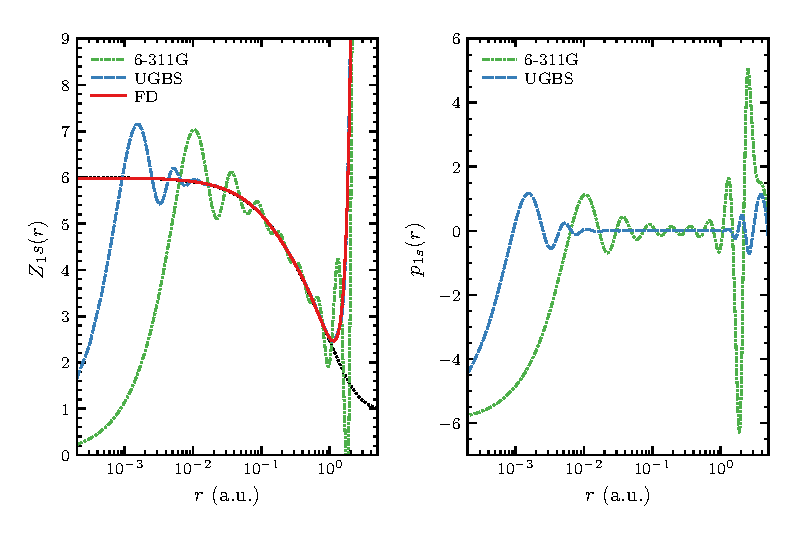
\includegraphics[width=0.9\textwidth]{dim/carbon_prof.eps}
\caption[Inversión de funciones de onda descritas con conjuntos de base.]
{(a) Cargas efectivas invertidas del orbital $1s$ del átomo de carbón.
(b) Perfiles de oscilación de los conjuntos de base.}
\label{fig:1sCarbon}
\end{figure}

Los patrones de oscilación varían según el conjunto de base utilizado
para representar las soluciones. Definimos los perfiles de oscilación
de cada BS como
\begin{equation}
 p_{nl}^{\mbox{\scriptsize BS}} = Z_{nl}^{\mbox{\scriptsize BS}}-
 Z_{nl}^{\mbox{\scriptsize FD}} \,,
 \label{eq:oscillation-prof}
\end{equation}
donde $Z_{nl}^{\mbox{\scriptsize BS}}$ es la carga invertida del átomo
cuando se usa el conjunto de bases ``BS'' y $Z_{nl}^{\mbox{\scriptsize FD}}$ 
es la carga efectiva que se obtiene a partir de la inversión de las 
soluciones del método de diferencias finitas. En el caso del carbono,
los conjuntos de base consideradas para calcular el orbital $1s$ fueron
\mbox{6-311G} y UGBS. Los perfiles de oscilación correspondientes a
dicho orbital, usando la ecuación~(\ref{eq:oscillation-prof}), 
se muestran en la figura~\ref{fig:1sCarbon}(b). Dado que los perfiles 
de oscilación para cada conjunto de base atómico son característicos,
una vez determinados, éstos pueden ser implementados para remover las
oscilaciones de los cálculos moleculares. 

Una vez que las oscilaciones son removidas de los cálculos moleculares, 
se procede a implentar el procedimiento de depuración descrito en la
sección~\ref{subsec:depuracion}. Debido a la 
estructura de las moléculas consideras, definimos una nueva ecuación 
parámetrica para las cargas moleculares DIM,
\begin{eqnarray}
 Z(r) = \sum_j z_j e^{-\alpha_j r} 
 + z_{\mbox{\scriptsize H}} e^{-(\ln r - \ln \beta)^2/(2\gamma)} 
 + 1\,.
 \label{eq:molzDIM}
\end{eqnarray}
En constraste con la aproximación propuesta para los 
átomos~(\ref{eq:atomzDIM}), incluimos un segundo término en la 
formula de ajuste para tener en cuenta la presencia de los hidrógenos en 
los compuestos hidruros. Esta expresión nos permite ajustar 
convenientemente tanto la ubicación como el ancho de los potenciales
hidrogénicos apantallados sin afectar el valor correcto de la carga en 
el origen.


%%%%%%%%%%%%%%%%%%%%%%%%%%%%%%%%%%%%%%%%%%%%%%%%%%%%%%%%%%%%%%%%%%%%%%%%
\section{Resultados}
%%%%%%%%%%%%%%%%%%%%%%%%%%%%%%%%%%%%%%%%%%%%%%%%%%%%%%%%%%%%%%%%%%%%%%%%

En esta sección, examinaremos los resultados obtenidos a partir de la 
implementación de nuestro método de potencial efectivo para la descripción 
de blancos atómicos y moleculares. 
La aplicabilidad del método de inversión depurada en blancos de 
estructura compleja es evaluada a través del estudio de la ionización 
por impacto de protones y fotones en átomos y moléculas. También 
analizaremos el desempeño de los potenciales DIM ante la primera 
aproximación de Born para predecir secciones eficaces totales de 
ionización de helio, nitrógeno, neón y metano.

%%%%%%%%%%%%%%%%%%%%%%%%%%%%%%%%%%%%%%%%%%%%%%%%%%%%%%%%%%%%%%%%%%%%%%%%
\subsection{Descripción de blancos colisionales}
%%%%%%%%%%%%%%%%%%%%%%%%%%%%%%%%%%%%%%%%%%%%%%%%%%%%%%%%%%%%%%%%%%%%%%%%
\subsubsection{Helio}
%%%%%%%%%%%%%%%%%%%%%%%%%%%%%%%%%%%%%%%%%%%%%%%%%%%%%%%%%%%%%%%%%%%%%%%%

En primer lugar, mostraremos los resultados obtenidos de implementar
el método de inversión depurada en el átomo de helio en su estado
fundamental. Dado que la inversión directa de este orbital no presenta 
ninguna de las complicaciones numéricas presentadas en la
sección~\ref{subsec:difnumericasDIM}; i.e., la función de onda del 
orbital $1s$ no tiene nodos y éste decae exponencialmente con la energía 
del orbital HOMO. Además, la simpleza del átomo de helio nos permite contar 
con un número reducido de parámetros necesarios para definir la carga 
efectiva DIM $Z_{1s}^{\mathrm{ DIM}}$ dada por la 
ecuación~(\ref{eq:atomzDIM}). Así, es posible optimizar esta función 
con sólo tres parámetros, los cuales se dan en la tabla~\ref{tab:parametrosHe}.

%%%%%%%%%%%%%% PARAMETROS CARGA EFECTIVA 
\begin{table}
\begin{center}
\begin{tabular}{|c|c|c|}
\hline
  $nl$ & $z$ & $\alpha$ \\
\hline
\hline
\multirow{2}{*}{$1s$} &  $1.31745$ & $2.50032$ \\
                      & $-0.31745$ & $5.04372$ \\
\hline
\end{tabular}
\caption[Parámetros de la carga efectiva del helio.]
{Parámetros de la carga efectiva $Z_{1s}^{\mathrm{ DIM}}$ del átomo de 
helio.}
\label{tab:parametrosHe}
\end{center}
\end{table}

Para verificar la calidad de las funciones de onda obtenidas, en la 
tabla~\ref{tab:resultadosHe} presentamos la comparación de las energías 
y los valores de radios medios obtenidos mediante el método de Inversión
Depurada, con sus correspondientes valores obtenidos utilizando el 
método de Hartree--Fock.

%%%%%%%%%%%% ENERGIAS Y VALORES MEDIOS DE HARTREE-FOCK E INVERSION 
\begin{table}
\begin{center}
\begin{tabular}{|c|c|c|c|c|}
\hline
$nl$ & & Energía & $\left<r\right>$ & $\left<1/r\right>$ \\
\hline
\hline
\multirow{2}{*}{$1s$} 
     &  HF  & -0.917956 & 0.927273 & 1.687282 \\
     & DIM  & -0.917956 & 0.927313 & 1.687251 \\
\hline
\end{tabular}
\caption[Energías y radios medios obtenidos con DIM y HF para helio.]
{Energías y radios medios del obtenidos con el método de Inversión 
Depurada y con el método de HF en helio.}
\label{tab:resultadosHe}
\end{center}
\end{table}

Como podemos ver, el potencial $V_{1s}^{\mathrm{ DIM}}$ es capaz de 
producir un orbital $\varphi_{1s}^{\mathrm{ DIM}}$ que tiene una 
energía que coincide con la energía original de HF en 6 cifras 
significativas. 
Los valores medios también muestran una concordancia espectacular, 
tanto para la región cercana al origen, como en los que muestrean 
la calidad de la región asintótica.

\begin{comment}
\begin{table}
\centering
\begin{tabular}{lccccccc}
\hline
\multirow{2}{*}{Método} 
 & \multirow{2}{*}{$nl$}
 & \multirow{2}{*}{$E$} 
 & \multirow{2}{*}{$\langle r\rangle$} 
 & \multirow{2}{*}{$\langle 1/r\rangle$}
 & \multicolumn{2}{c}{Parámetros}  \\
 &  &  & & & $z$ & $\alpha$ \\
\hline
\arrayrulecolor{gray!30!white}
\hline
\multirow{2}{*}{Ajuste manual} 
 & \multirow{2}{*}{$1s$} & \multirow{2}{*}{$-0.91796$} % -3.216e-05
                         & \multirow{2}{*}{$0.92731$}  % -4.269e-03
                         & \multirow{2}{*}{$1.68725$}  %  1.830e-03  J= 0.0061
\hline
\multirow{2}{*}{Hartree--Fock} 
 & \multirow{2}{*}{$1s$} & \multirow{2}{*}{$-0.91796$} 
                         & \multirow{2}{*}{$0.92727$}
                         & \multirow{2}{*}{$1.68728$} & & \\
\\
\arrayrulecolor{black}\hline
\end{tabular}
\caption[Comparación de observables según ajuste de la carga efectiva de helio.]
{Comparación de energía y valores medios de la función de onda del 
orbital $1s$ de helio obtenidos mediante la diagonalización de la carga
efectiva $Z_{1s}^{\mathrm{DIM}}$. Los parámetros que definen la carga
se obtienen mediante la optimización manual.}
\label{tab:params-helio}
\end{table}
\end{comment}

%%%%%%%%%%%%%%%%%%%%%%%%%%%%%%%%%%%%%%%%%%%%%%%%%%%%%%%%%%%%%%%%%%%%%%%%
\subsubsection{Nitrógeno}
%%%%%%%%%%%%%%%%%%%%%%%%%%%%%%%%%%%%%%%%%%%%%%%%%%%%%%%%%%%%%%%%%%%%%%%%

La configuración más baja del nitrógeno $2p^3$ da lugar a tres términos
diferentes: $2\,^4$S, $2\,^2$D, $2\,^2$P. Cada uno de estos términos 
está descrito por una densidad electrónica diferente. Los parámetros 
que definen las cargas efectivas para cada término están dados en la 
tabla~\ref{tab:parametersNitro}. Resolviendo la ecuación (\ref{eq:Schrodinger}) 
con las cargas efectivas DIM definidas es posible reproducir los valores 
medios $\langle r \rangle$ y $\langle 1/r \rangle$ hasta en un $0.2\%$ 
de los valores de Hartree--Fock. Más aún, las energías totales DIM para 
cada término reproducen las originales hasta $10^{-4}\%$. 

\begin{figure}
\centering
\includegraphics[width=0.9\textwidth]{figures/dim/N_dim.eps}
\caption[Cargas efectivas DIM de nitrógeno.]
{Cargas efectivas del término $2\,^4$S de N; 
inversión directa (lineas discontinuas) 
e inversión depurada (líneas sólidas).}
\label{fig:Nzeff}
\end{figure}

\begin{table}
\centering
\begin{tabular}{|c|c|c|c|c|c|c|}
\hline
\multirow{2}{*}{$nl$} 
  & \multicolumn{2}{c}{$2\,^4$S} 
  & \multicolumn{2}{c}{$2\,^2$D} 
  & \multicolumn{2}{c}{$2\,^2$P} \\
\cline{2-7}
       & $z$ & $\alpha$ 
       & $z$ & $\alpha$ 
       & $z$ & $\alpha$ \\
\hline
\hline
\multirow{2}{*}{$1s$} & 5.25634  & 1.26207 
       & 5.18635  & 1.22410
       & 5.18635 & 1.21779  \\
\vspace*{0.09cm}
       & 0.743660 & 8.02844 
       & 0.813650 & 7.56800
       & 0.813650 & 7.56740   \\
       %%%%%%%%%%%%%%%%%%%%%%%%%%%%%%%%%
\hline
\multirow{3}{*}{$2s$} & 2.45281  & 3.51271 
       & 0.398100 & 0.239738
       & 0.890660 & 0.830615  \\
       & 0.833570  & 3.38654 
       & 1.85412  & 1.03105
       & 3.66999  & 3.14946   \\
\vspace*{0.09cm}
       & 2.71362  & 0.894699 
       & 3.74778  & 2.85313
       & 1.43935  & 0.740427  \\
       %%%%%%%%%%%%%%%%%%%%%%%%%%%%%%%%%
\hline
\multirow{3}{*}{$2p$}  & 3.64345  & 1.24069 
       & 4.01052  & 1.28744
       & 1.89769  & 1.16557  \\
       & 2.05501  & 5.35135 
       & 1.85517  & 5.70858 
       & 1.77430   & 5.68782 \\
       & 0.301540 & 0.286609 
       & 0.134310  & 0.267987
       & 2.32801  & 1.40925  \\
\hline
\end{tabular}
\caption[Parámetros de ajuste de cargas efectivas de nitrógeno.]
{Parámetros de ajuste de las cargas efectivas 
$Z_{nl}^{\mathrm{DIM}}(r)$ para los términos $2\,^4$S, $2\,^2$D y
$2\,^2$P del nitrógeno.}
\label{tab:parametersNitro}
\end{table}

\begin{table}
\centering
\begin{tabular}{|c|c|c|c|c|c|}
\hline
   & $nl$ &  $\epsilon$  
   & $\langle r \rangle$
   & $\langle 1/r \rangle$ 
   & $\langle r^2 \rangle$ \\ 
\hline
\hline
\multirow{6}{*}{$2\,^4$S}
   & \multirow{2}{*}{$1s$} 
          & -15.629060 & 0.228296 & 6.648629 & 0.070199 \\
   &      & -15.629060 & 0.22830  & 6.65324  & 0.07027  \\
\cline{2-6}
   & \multirow{2}{*}{$2s$}
          & -0.945324  & 1.334474 & 1.080369 & 2.145339 \\
   &      & -0.945324  & 1.33228  & 1.07818  & 2.14944  \\
\cline{2-6}
   & \multirow{2}{*}{$2p$}
          & -0.567589  & 1.412683 & 0.954982 & 2.555457 \\
   &      & -0.567589  & 1.40963  & 0.95769  & 2.54766  \\
\hline
%%%%%%%%%%%%%%%%%%%%%%%%%%%%%%%%%%%%%%%%%%%%%%%%%%%%%%%%%%%%%%
\multirow{6}{*}{$2\,^2$D}
   & \multirow{2}{*}{$1s$}
          & -15.666392 & 0.228290 & 6.649289 & 0.070200 \\
   &      & -15.666392 & 0.22826  & 6.65388  & 0.07024  \\
\cline{2-6}
   & \multirow{2}{*}{$2s$}
          & -0.963670  & 1.329174 & 1.086439 & 2.134548 \\
   &      & -0.963670  & 1.32632  & 1.08318  & 2.12941  \\
\cline{2-6}
   & \multirow{2}{*}{$2p$}
          & -0.508655  & 1.448778 & 0.938821 & 2.709128 \\
   &      & -0.508655  & 1.44662  & 0.94208  & 2.70716  \\
\hline
%%%%%%%%%%%%%%%%%%%%%%%%%%%%%%%%%%%%%%%%%%%%%%%%%%%%%%%%%%%%%%
\multirow{6}{*}{$2\,^2$P}
   & \multirow{2}{*}{$1s$}
          & -15.691599 & 0.228242 & 6.650362 & 0.070167 \\
   &      & -15.691599 & 0.22824  & 6.65430  & 0.07022  \\
\cline{2-6}
   & \multirow{2}{*}{$2s$}
          & -0.976339  & 1.325618 & 1.087123 & 2.115849 \\
   &      & -0.976339  & 1.32232  & 1.08656  & 2.11600  \\
\cline{2-6}
   & \multirow{2}{*}{$2p$}
          & -0.471297  & 1.471755 & 0.929822 & 2.811999 \\
   &      & -0.471297  & 1.47301  & 0.93155  & 2.82518  \\
\hline
\end{tabular}
\caption[Energías y valores medios orbitales de nitrógeno.]
{Energías orbitales y valores medios de los términos 
$2\,^4$S, $2\,^2$D y $2\,^2$P de N, obtenidos mediante potentiales 
efectivos DIM (filas superiores) y el método de Hartree--Fock (filas 
inferiores).} 
\label{tab:resultsNitro}
\end{table}

%%%%%%%%%%%%%%%%%%%%%%%%%%%%%%%%%%%%%%%%%%%%%%%%%%%%%%%%%%%%%%%%%%%%%%%%
\subsubsection{Neón}
%%%%%%%%%%%%%%%%%%%%%%%%%%%%%%%%%%%%%%%%%%%%%%%%%%%%%%%%%%%%%%%%%%%%%%%%

\newpage
%%%%%%%%%%%%%%%%%%%%%%%%%%%%%%%%%%%%%%%%%%%%%%%%%%%%%%%%%%%%%%%%%%%%%%%%
\subsubsection{Metano}
%%%%%%%%%%%%%%%%%%%%%%%%%%%%%%%%%%%%%%%%%%%%%%%%%%%%%%%%%%%%%%%%%%%%%%%%

Implementamos el método de Inversión Depurada en la molécula de metano,
ya que es ésta es altamente simétrica y, por lo tanto, puede ser descrita
por un potencial angular promediado~\cite{Granados:16}. Calculamos los 
orbitales moleculares de HF de CH$_4$ usando los conjuntos de bases 
UGBS del carbono y el hidrógeno, los cuales consideran momentos angulares
hasta $L=1$. Los cálculos de metano con estos conjuntos de base deberían
incluir funciones de polarización (por lo menos hasta las funciones $d$)
para incrementar la precisión de las energías
 moleculares~\cite{Rothenberg:71,Hariharan:72}. Sin embargo, para
aislar los efectos de los conjuntos de base, realizamos los cálculos de 
perfiles de oscilación descritos en la sección~\ref{subsec:invdepGTO} y 
los orbitales moleculares en el mismo esquema. Las cargas obtenidas 
mediante la inversión directa se muestran en la figura~\ref{fig:ch4zeff} 
con líneas discontinuas. Dado que los orbitales moleculares están 
escritos por combinaciones lineales de orbitales atómicos del carbono
y el hidrógeno, las oscilaciones de las cargas invertidas se deben al 
número finito de funciones primitivas en el conjunto de base de cada átomo.
Para remover estas oscilaciones, se deben determinar los perfiles de 
oscilación producidas por el conjunto de base del carbono. Usamos la 
ecuación~(\ref{eq:oscillation-prof}) para determinar los perfiles
$p_{1s}^{\mbox{\scriptsize UGBS}}$, $p_{2s}^{\mbox{\scriptsize UGBS}}$ 
y $p_{2p}^{\mbox{\scriptsize UGBS}}$ del carbono. Así, se puden remover
los perfiles $p_{nl}^{\mbox{\scriptsize UGBS}}$ de las correspondientes
cargas invertidas $Z_{i}^{\mbox{\scriptsize UGBS}}$ del metano. Las
oscilaciones son completamente removidas para todos los orbitales 
excepto el $2a_2$, que presenta pequeñas fluctuaciones residuales debido
a la base del hidrógeno. Ya que estas ondulaciones son mínimas y se 
ubican cerca del núcleo, procedemos a implementar le método de 
depuración descrita en la sección~\ref{subsec:invdepGTO}. 

Los parámetros optimizados de las cargas moleculares DIM de metano y los
valores de energía obtenidos con ellas se dan en la 
tabla~\ref{tab:ch4parameters}. Las cargas correspondientes se muestran 
en la figura~\ref{fig:ch4zeff} con líneas sólidas. 

\begin{figure}
\centering
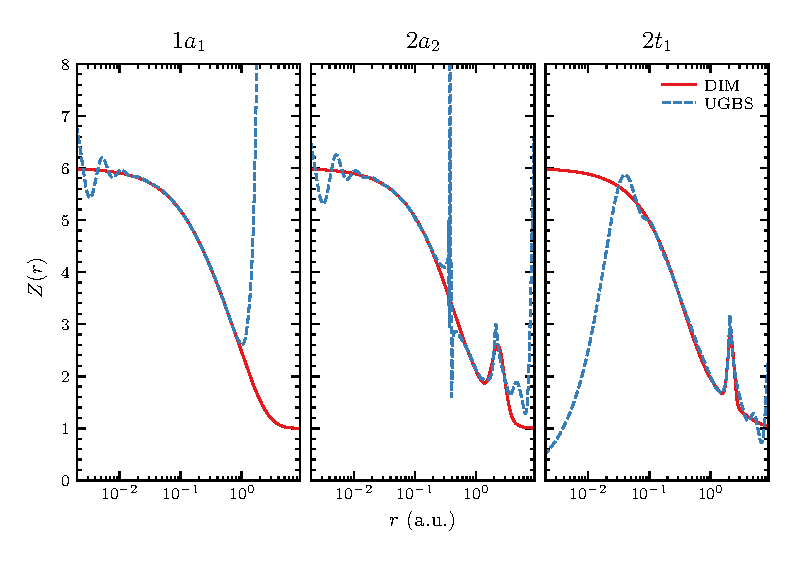
\includegraphics[width=0.9\textwidth]{figures/dim/ch4_dim.eps}
\caption[Cargas efectivas DIM de metano.]
{Cargas efectivas de CH$_4$; inversión directa (lineas discontinuas)
e inversión depurada (líneas sólidas).}
\label{fig:ch4zeff}
\end{figure}

\begin{table}
\centering
\begin{tabular}{|c|c|c|c|c|c|c|}
\hline
   $nl$ & $E$ &$z$ & $\alpha$ & $z_{\mbox{\scriptsize H}}$ & $\beta$ & $\gamma$ \\
\hline
\hline
\multirow{3}{*}{$1a_1$} 
  & \multirow{3}{*}{-11.1949}
      & 1.925280 & 0.641982 & & & \\
    & & 0.953120 & 5.571510 & & & \\
    & & 2.121600 & 1.500440 & & & \\
\hline
\multirow{2}{*}{$2a_2$}
 & \multirow{2}{*}{-0.9204}
      & 2.912200 & 3.149990 & \multirow{2}{*}{1.23640} & \multirow{2}{*}{2.329570} & \multirow{2}{*}{0.053420} \\
    & & 2.087800 & 0.771371 & & & \\
\hline
\multirow{3}{*}{$2t_1$}
 & \multirow{3}{*}{-0.5042}
      & 0.901953 & 2.895140 & \multirow{3}{*}{1.30182} & \multirow{3}{*}{2.169850} & \multirow{3}{*}{0.012616} \\
    & & 1.112030 & 0.388649 & & & \\
    & & 2.986017 & 2.931210 & & & \\
\hline
\end{tabular}
\caption[Energías y parámetros de ajuste de cargas efectivas de metano.]
{Energías orbitales moleculares y parámetros de ajuste de cargas efectivas
dadas por la ecuación~(\ref{eq:molzDIM}) de metano.}
\label{tab:ch4parameters}
\end{table}

\newpage
%%%%%%%%%%%%%%%%%%%%%%%%%%%%%%%%%%%%%%%%%%%%%%%%%%%%%%%%%%%%%%%%%%%%%%%%
\subsection{Fotoionización}
\label{subsec:foto}

En esta sección analizaremos la respuesta del potencial efectivo DIM, 
obtenido mediante el método de inversión depurada, ante el proceso de
fotoionización para tres blancos atómicos: helio, nitrógeno y neón. 
Los átomos, con estado de carga neutro, son estudiados en sus estados
fundamentales.

Empleando la primera aproximación de Born (FBA), las secciones eficaces
total de fotoionización de los átomos de helio, nitrógeno y neón descritos 
mediante los potenciales DIM se muestran con líneas sólidas en las 
figuras~\ref{fig:HephotoDIM}, \ref{fig:NphotoDIM} y \ref{fig:NephotoDIM}.
Los datos experimentales~\cite{Henke:93,Samson:90,Samson:02,Stolte:16} 
se muestran con símbolos. Denominamos la combinación de la 
descripción del blanco mediante el potencial efectivo DIM y la descripción 
de la fotoionización a primer orden como fotoionización DIM. 
Las secciones eficaces totales de la fotoionización DIM para ambos 
blancos coinciden de manera excelente con los valores experimentales
a bajas, medias y altas energías del fotón incidente. Para el átomo de
neón, algunas discrepancias empiezan a surgir a energías bajas e 
intermedias del projectil. Este comportamiento sugiere la necesidad de 
incluir en la descripción de la fotoionización correcciones de mayor 
orden que incluyan efectos de múltiples cuerpos que puedan ser 
relevantes tales como la relajación de los orbitales debido a la 
creación de un hueco electrónico, respuestas colectivas de electrones 
de capas internas~\cite{Ederer:64} y efectos de correlación.

\begin{figure}[H]
\centering
 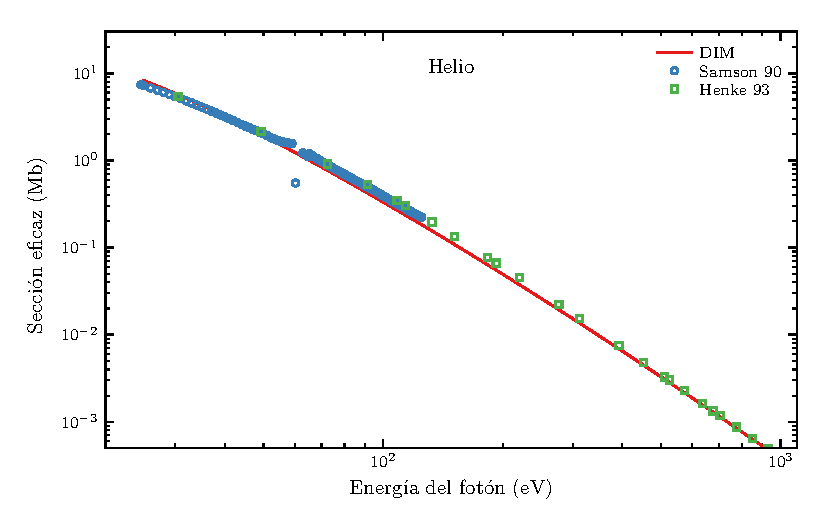
\includegraphics[width=0.9\textwidth]{dim/He_fotoDIM.eps}
\caption[Fotoionización de helio.]
{Sección eficaz total de fotoionización de un electrón del helio}
\label{fig:HephotoDIM}
%\end{figure}
%\begin{figure}[H]
%\centering
\vspace{0.5cm}
 \includegraphics[width=0.9\textwidth]{dim/N_fotoDIM.eps}
\caption[Fotoionización de nitrógeno.]
{Sección eficaz total de fotoionización de un electrón del 
nitrógeno.}
\label{fig:NphotoDIM}
\end{figure}
\begin{figure}[H]
\centering
 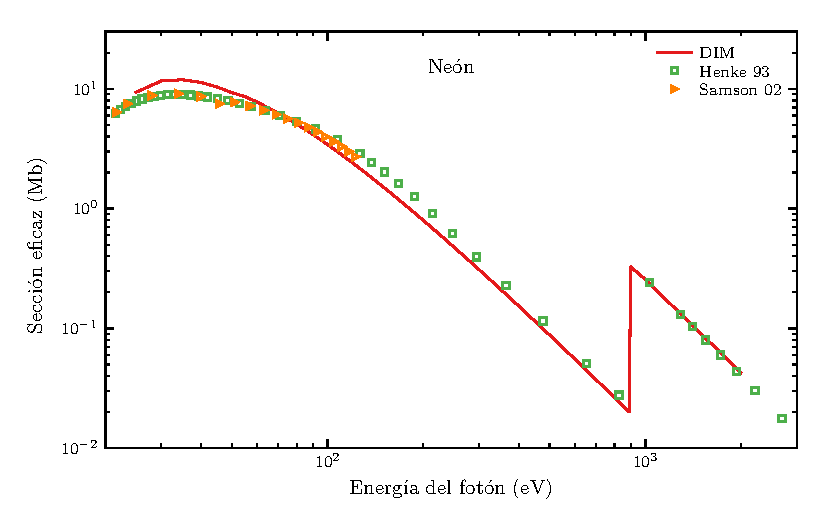
\includegraphics[width=0.9\textwidth]{dim/Ne_fotoDIM.eps}
\caption[Fotoionización de neón.]
{Sección eficaz total de fotoionización de un electrón del neón.}
\label{fig:NephotoDIM}
\end{figure}

La sección eficaz total de fotoionización de CH$_4$, basadas en la 
descripción del blanco molecular con el potencial DIM y la primera 
aproximación de Born, se muestra en la figura~\ref{fig:photoch4} con 
líneas sólidas. Se encuentran buen acuerdo con los resultados 
experimentales, los cuales se muestran con símbolos, en el rango de
altas energías y cerca del umbral. La curva entre $\sim$15 y 
$\sim$300 eV muestra la fotoionización de la capa eterna $n=2$, mientras
que la discontinuidad en 300 eV corresponde al umbral del orbital 
molecular $1a_1$. Para fotoenergías bajas e intermedias, el acuerdo entre 
nuestras predicciones y los datos 
experimentales~\cite{Lukirskii:64,Henke:82,Samson:89} no es muy bueno.
Fenónemos tales como la relajación de los orbitales moleculares, posibles
contribuciones colectivas y efectos de correlación deben ser considerados 
en futuros cálculos. Por otro lado, para la fotoionización de un electrón
perteneciente al orbital interno $1a_1$, estos efectos no son tan 
signficativos, y obtenemos buen acuerdo con los valores experimentales
disponibles.

\begin{figure}[t]
\centering
 \includegraphics[width=0.9\textwidth]{figures/dim/ch4_fotoDIM.eps}
\caption[Fotoionización de metano.]
{Sección eficaz total de fotoionización de un electrón de la
molécula de metano. Línea sólida: cálculos teóricos a primer orden de 
aproximación con potencial molecular DIM. Símbolos: experimentos de 
Refs.~\cite{Lukirskii:64,Henke:82,Samson:89}.}
\label{fig:photoch4}
\end{figure}

\subsection{Ionización por impacto de protón}

\begin{figure}[t]
\centering
 \includegraphics[width=0.9\textwidth]{figures/dim/ch4_ionDIM.eps}
\caption[Ionización de metano por impacto de protón.]
{Sección eficaz total de ionización de un electrón de la
molécula de metano por impacto de protón. Línea sólida: cálculos 
teóricos a primer orden de aproximación con potencial molecular DIM. 
Símbolos: experimentos de Refs.~\cite{Rudd:83,Rudd:85}.}
\label{fig:ionch4}
\end{figure}

\newpage
%=======================================================================
\section{Conclusiones}
\label{conclusion}

En esta sección, exploramos la implementación de un método de Inversión
Depurada para obtener potenciales efectivos que permitan describir
blancos atómicos y moleculares de manera precisa en el marco del modelo 
de electrón activo. La disponibilidad de tales potenciales efectivos 
permite conocer los estados iniciales y finales en procesos colisonales 
de manera directa. Se utilizó la primera aproximación de Born para 
calcular ionización por impacto de protones y fotones. 

Se estudiaron tres sistemas atómicos: helio, nitrógeno y neón. El método 
de Inversión Depurada permite obtener potenciales efectivos que 
reproducen los valores de HF de forma precisa. A su vez, los potenciales
DIM permiten predecir resultados experimentales de secciones eficaces
de ionización en un amplio rango de energías del proyectil incidente.

El método de Inversión depurada para átomos fue extendido para la 
obtención de potenciales moleculares efectivos. Debido a que los 
orbitales moleculares se expresan usando conjuntos de base finitas, 
la implementación de la inversión traduce pequeñas fluctuaciones en las
soluciones de HF en grandes oscilaciones en la carga molecular.
Debido a esto, se requieren pasos adicionales en el método de depuración,
los cuales incluyen la determinación de perfiles de oscilación de los
conjuntos de base atómicas utilizadas en el cálculo molecular.
Usamos el método de Inversión Depurada para determinar potenciales
efectivos para CH$_4$. Los potenciales son implementados para obtener
los estados iniciales y finales en procesos de ionización a primer orden
por impacto de protones y fotones. Ambos procesos son reproducidos en 
términos generales con buena concordancia con los datos experimentales 
disponibles. Las discrepancias principales se atribuyen al hecho de 
que nuestro cálculo sólo considera el primer orden perturbativo.




